%!TEX root = main.tex
\section{Results}

The Dieleman model was used for both sex and speaker classification. In addition the baseline of choosing the largest class, a logistic regression model applied to the mean frequencies and a GMM is included for comparison. The results for sex and speaker classification is included below:
\begin{table}[H]
\centering
\begin{tabular}{r|c|c}
model & TIMIT & ELSDSR \\ \hline
                    Baseline & $0.354$ & $0.465$ \\
                    Logistic on mean & $0.094 \pm 0.012$ & $0.030 \pm 0.007$ \\
                 GMM on MFCC & $0.192 \pm 0.024$ & $0.140 \pm 0.019$ \\
                    Dieleman & $0.093 \pm 0.012$ & $0.026 \pm 0.006$ \\
     Dieleman + L2 & $0.114 \pm 0.013$ & $0.036 \pm 0.016$ \\
  Dieleman + Scale & $0.111 \pm 0.015$ & $0.022 \pm 0.006$ \\
 Dieleman + Offset & $0.107 \pm 0.008$ & $0.027 \pm 0.014$ \\
\end{tabular}
\caption{Misclassification rates for sex classification with $95\%$ confidence intervals.}
\label{tab:results-sex}
\end{table}

\begin{table}[H]
\centering
\begin{tabular}{r|c|c}
model & TIMIT & ELSDSR \\ \hline
                    Baseline & $0.988$ & $0.957$ \\
                    Logistic on mean & $0.796 \pm 0.046$ & $0.338 \pm 0.043$ \\
                 GMM on MFCC & $0.836 \pm 0.020$ & $0.391 \pm 0.023$ \\
                    Dieleman & $0.965 \pm 0.021$ & $0.570 \pm 0.029$ \\
     Dieleman + L2 & $0.944 \pm 0.020$ & $0.552 \pm 0.045$ \\
  Dieleman + Scale & $0.973 \pm 0.007$ & $0.640 \pm 0.110$ \\
 Dieleman + Offset & $0.971 \pm 0.006$ & $0.628 \pm 0.117$ \\
\end{tabular}
\caption{Misclassification rates for speaker classification with $95\%$ confidence intervals.}
\label{tab:results-speaker}
\end{table}

As seen the Dieleman model does not appear to be better than a simple logistic model or the GMM. Because the logistic model can be expressed as a simple neural network, it was attempted to increase the depth of the logistic network one layer at a time to form the Dieleman network. However, all variations that used convolutional layers had performance similar to the Dieleman network.

The regularization parameter for Weight Decay (L2) in the speaker classification was optimized. Similar procedure could have been done on the Scale Invariant and Offset Invariant regularizers, however the implementation of those where so slow that we considered it infeasible for the Dieleman network.

\begin{figure}[H]
  \centering
  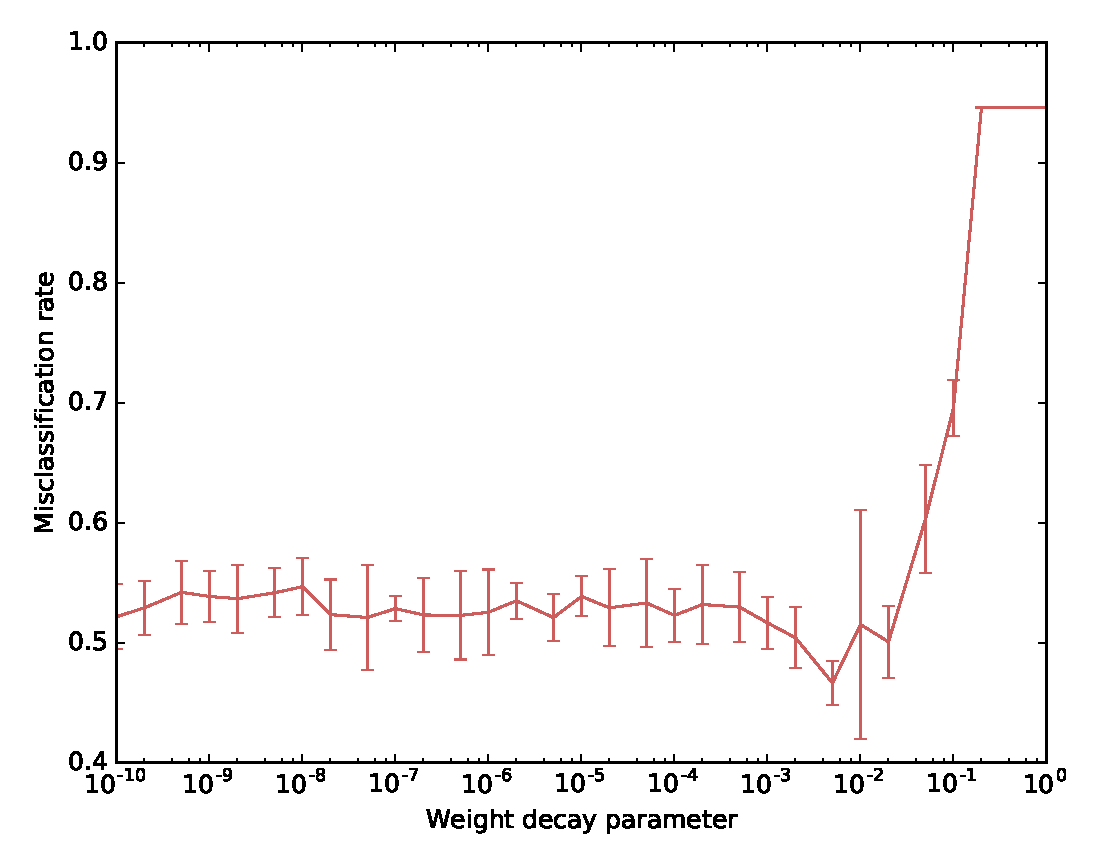
\includegraphics[width=0.4\textwidth]{plots/reg_opt_dieleman_speaker_elsdsr}
  \caption{Weight decay optimization for the speaker classification problem on the ELSDSR dataset, using $5$-fold cross-validation.}
  \label{fig:reg_opt}
\end{figure}

The best regularizer parameter is $\lambda = 5 \cdot 10^{-3}$. To ensure it is statistically significantly different from choosing $\lambda = 0$ a two-sample t-test was used. This yields $p = 0.00070$, i.e. we can reject the null hypothesis $\lambda=0$ at a $5\%$ significance level. A 20-fold CV was performed on a finer grid around $\lambda = 5 \cdot 10^{-3}$ in \cref{appendix:optimization-weight-decay}.

\subsection{Synthetic datasets}

The invariance regularizers seemed to have a no impact (or negative impact) on sex and speaker classification. Thus 4 synthetic data generators were constructed to test if invariance had potential in other areas:
\begin{itemize}
\item{Circles: A generator creating two circle of different clases slightly overlapping each other.}
\item{Linear: Two linearly seperable classes.}
\item{Moons: Two half-moons intertwined with each other}
\item{XOR: The binary xor in 2d.}
\end{itemize}

For each data generator the optimal regularization parameters where chosen. This was done by sampling 10 datasets per generator, model and regularization choice. The results can be seen in \cref{appendix:regualization-optimization}. The best parameters were then used to compare the models, see \cref{fig:2d_significant}.

\begin{figure}[h]
	\centering
	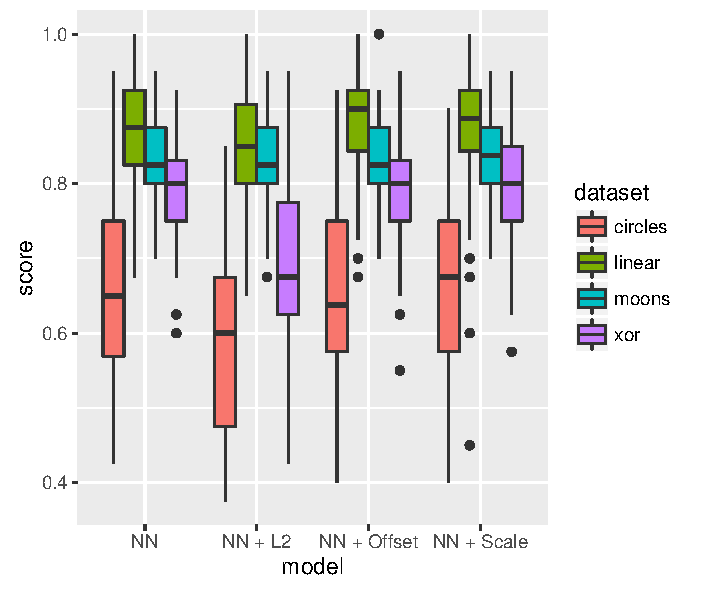
\includegraphics[width=0.45\textwidth]{plots/2d_significant}
	\caption{Boxplot of misclassification rate over 100 datasets.}
	\label{fig:2d_significant}
\end{figure}

As seen from \cref{fig:2d_significant} there is no significant benefit from using any of the regularizers. However, misclassification is only affected by the decision boundary and thus there might differences in the estimated probability function. But when inspecting the contours (see \cref{appendix:generated-contour-optimized}) no such differences could be observed. Finally, the regularizers parameters were set to extreme values to check if the regularizers had any influence on the contours (see \cref{plt:generated-contour-extream}).

\begin{figure*}[ht]
	\centering
	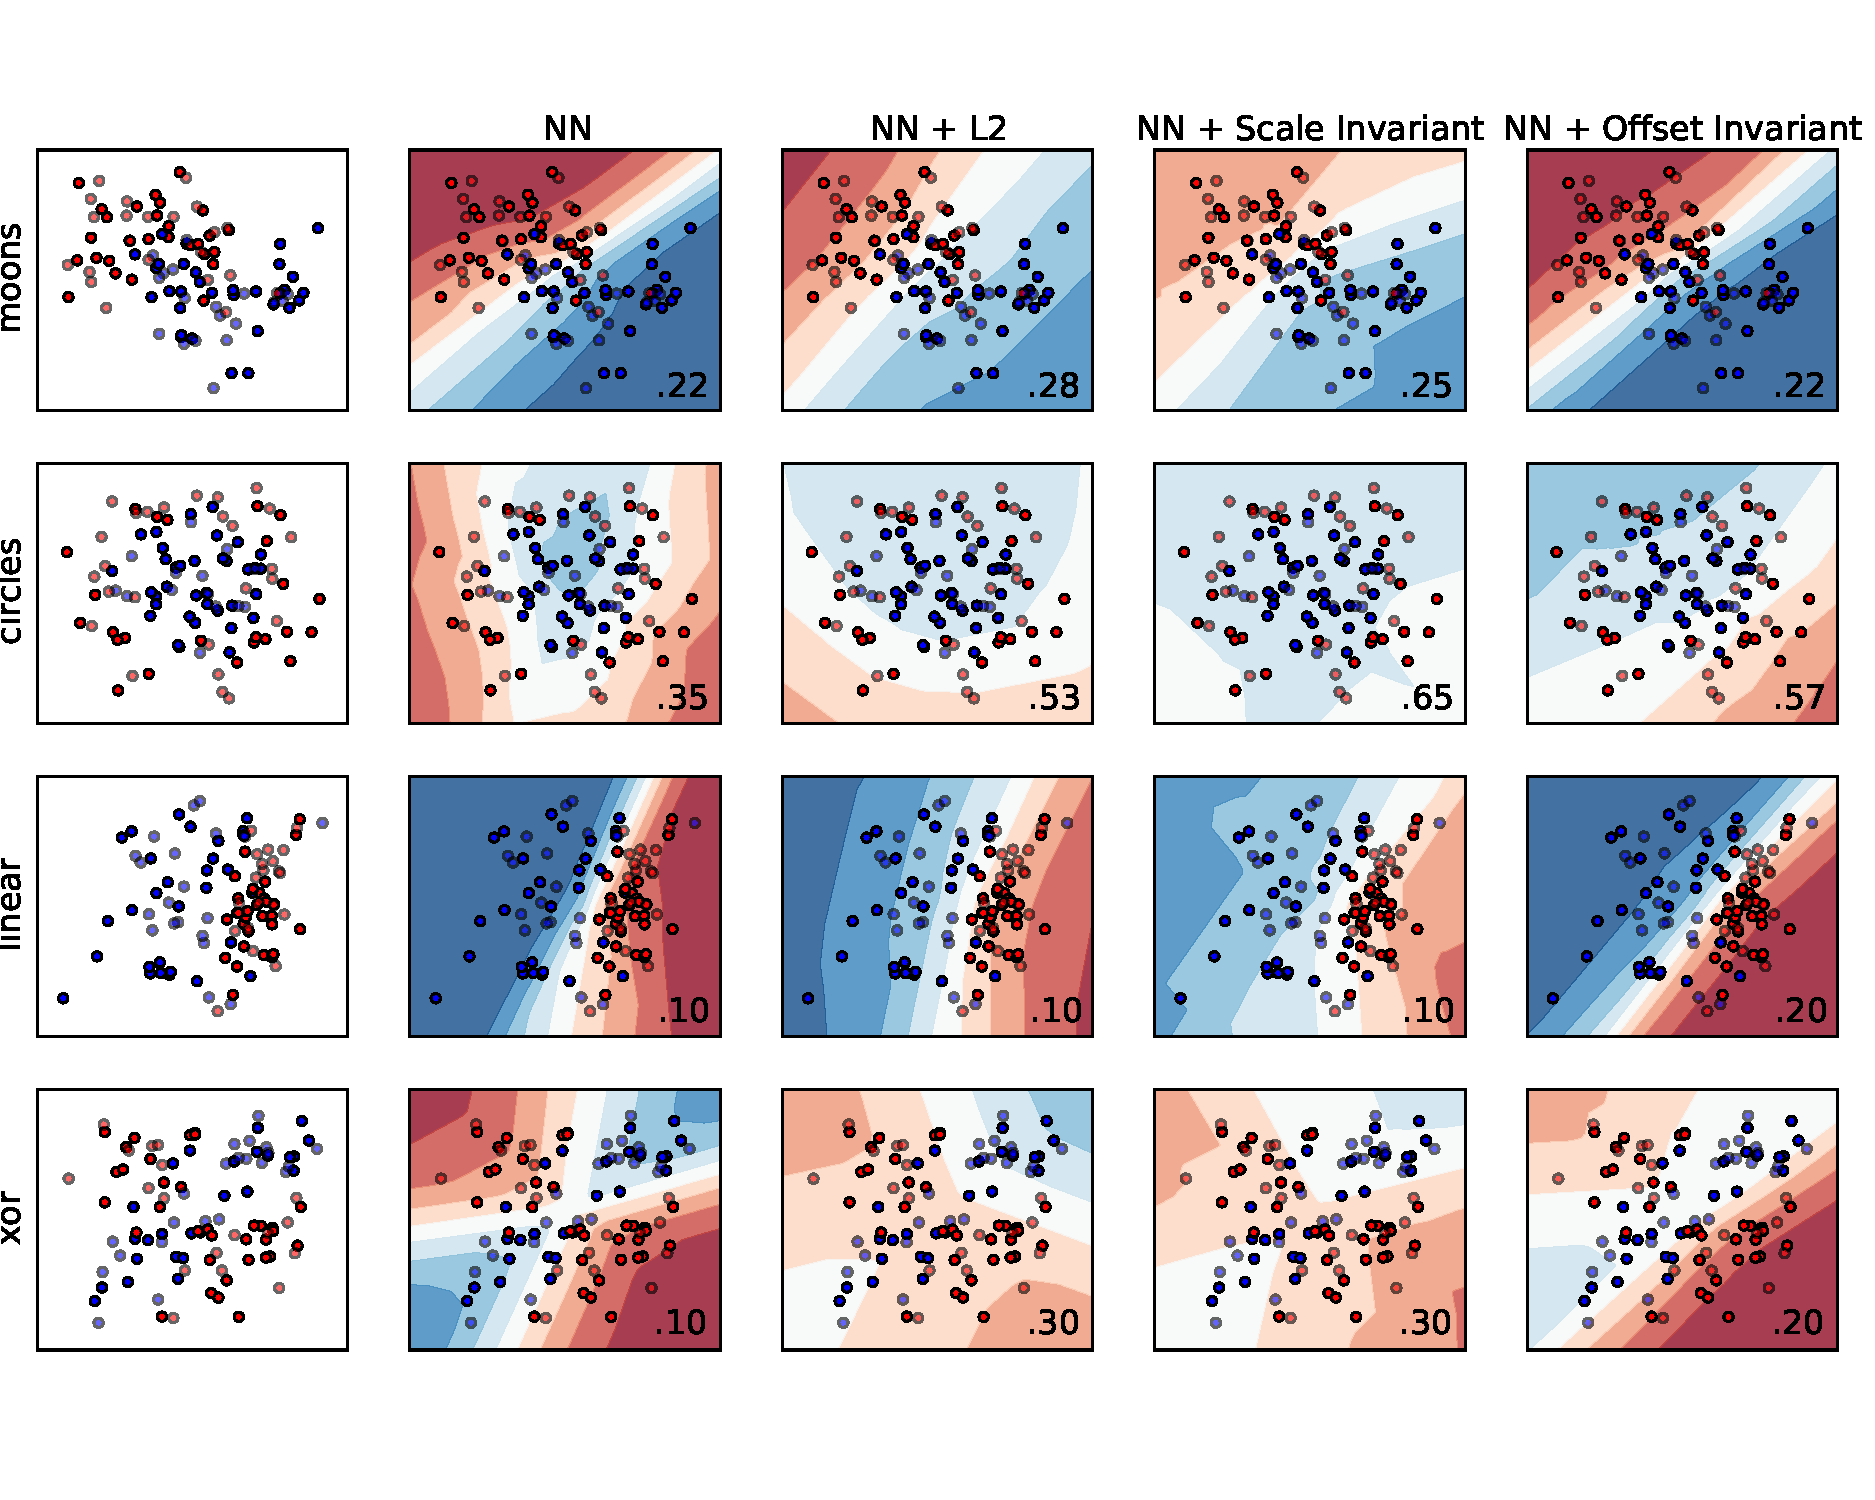
\includegraphics[width=0.7\textwidth, trim = 0 2.2cm 0 1.5cm, clip]{plots/2d_classifier-extream}
	\caption{Observations and contour plots of the class probability function for each classifier and dataset. The regularizers's parameters were set to extreme values to make their influence visible. $0.1$ for \textit{NN + L2} and $10$ for \textit{NN + Scale/Offset Invariant}.}
	\label{plt:generated-contour-extream}
\end{figure*}
